\documentclass[tikz,border=8pt]{standalone}
% Shared look for every TikZ diagram. Load with \input{../../tools/tikz-style.tex}
\usepackage[T1]{fontenc}
\usepackage{lmodern}
\renewcommand{\sfdefault}{lmr}  % diagrams use the same serif as the text
\usetikzlibrary{arrows.meta, positioning, shapes.geometric, calc, fit, backgrounds}
\definecolor{cblue}{HTML}{4C78A8}
\definecolor{corange}{HTML}{F58518}
\definecolor{cgreen}{HTML}{54A24B}
\definecolor{cred}{HTML}{E45756}
\definecolor{cpurple}{HTML}{B279A2}
\definecolor{cgrey}{HTML}{6B6B6B}
\tikzset{
  every picture/.style={font=\sffamily, line width=1.2pt},
  box/.style={draw=#1, fill=#1!12, rounded corners=4pt, align=center, inner sep=7pt, minimum height=1.1cm},
  box/.default=cgrey,
  arrow/.style={-{Stealth[length=3mm]}, draw=cgrey, line width=1.4pt},
  title/.style={font=\sffamily\bfseries\Large},
  note/.style={font=\sffamily\small, text=cgrey, align=center},
}
\AtBeginDocument{\hyphenpenalty=10000 \exhyphenpenalty=10000}

% The L-shaped cabinet is not convex: the segment between two of its points can leave it. It is the union of two
% rectangles R1 = [5.6, 7] x [3.4, 4] and R2 = [6.4, 7] x [2.4, 4], each an intersection of four half-planes.
\begin{document}
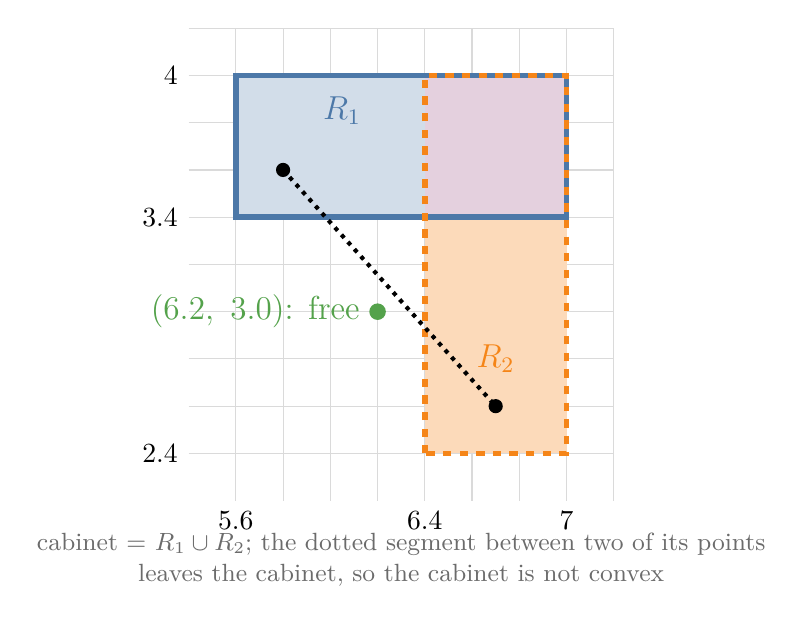
\begin{tikzpicture}[scale=3, every node/.append style={font=\large}]
  \draw[cgrey!25, line width=0.4pt] (5.4,2.2) grid[step=0.2] (7.2,4.2);
  \fill[cblue!25] (5.6,3.4) rectangle (7,4);
  \fill[corange!30] (6.4,2.4) rectangle (7,4);
  \fill[cpurple!35] (6.4,3.4) rectangle (7,4);
  \draw[cblue, line width=2pt] (5.6,3.4) rectangle (7,4);
  \draw[corange, line width=2pt, dashed] (6.4,2.4) rectangle (7,4);
  \node[cblue] at (6.05,3.85) {$R_1$}; \node[corange] at (6.7,2.8) {$R_2$};
  \fill[cgreen] (6.2,3.0) circle (0.035); \node[cgreen, left] at (6.17,3.0) {$(6.2,\ 3.0)$: free};
  \fill[black] (5.8,3.6) circle (0.03); \fill[black] (6.7,2.6) circle (0.03);
  \draw[black, dotted, line width=1.5pt] (5.8,3.6) -- (6.7,2.6);
  \node[note, align=center] at (6.3,1.95) {cabinet = $R_1 \cup R_2$; the dotted segment between two of its points\\leaves the cabinet, so the cabinet is not convex};
  \foreach \t in {5.6,6.4,7} \node[below, font=\normalsize] at (\t,2.2) {\t};
  \foreach \t in {2.4,3.4,4} \node[left, font=\normalsize] at (5.4,\t) {\t};
\end{tikzpicture}
\end{document}
